\chapter{Dependency Modelling}
\label{chap:dependencies}

\section{Scaling and allocating claims}
\label{sec:scalingClaims}
If an attritional claim is simply a fraction of another claim, then this is a dependency structure, albeit a very simple one. Of course, we could explicitly re-scale the claims distribution and capture the new distribution parameters. But for various reasons this may not always be the best solution. If for example we get market loss\index{market loss} distributions from an external provider, then for review and audit reasons we capture these original parameters and scale the claims to the appropriate scale of the portfolio. Another reason may be that the same claims source is used with different scalings in different parts of a model. And a third application is if one quickly wants to perform a simple sensitivity analysis\index{sensitivity analysis} with respect to a claims distribution.

Figure~\ref{fig:ScalingClaims} shows that scaling factors\index{scaling factor} are entered in the multi-dimensional parameter called Share. This multi-dimensional parameter is used to associate the claims generators to the lines of business and set their scaling factors. 
\begin{figure}
		\centering
		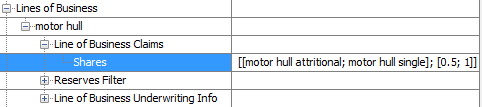
\includegraphics{images/scalingClaims.png}\\[5mm]
				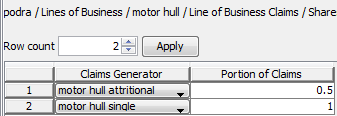
\includegraphics{images/scalingClaimsDetails.png}
	\caption{Scaling or allocating claims}
	\label{fig:ScalingClaims}
\end{figure}
The term Share suggests another use of this scaling: Parts of a claims can be allocated to different lines of business. This may be necessary if policies cover multiple risks, but the historic data may not be sufficient to calibrate claims distributions for each risk which are covered by the policy. In the cases in which we talk about allocating claims to multiple lines of business their shares usually add up to 1. This is not the case if for example a market loss is scaled. In fact, in some cases scaling factors which are greater than 1 may make sense. Hence, there is no validator which checks that the shares add up to 1 and/or each share is less than 1. 


\section{Dependency models for attritional claims}
\label{sec:depAttritional}
Copulas offer a way to construct joint distributions with given marginals. This is a frequently encountered problem in actuarial work. If one cause leads to several different claim types, \eg property damage and fire following, then there exists a \ix{copula!}{joint distribution} of these claims. If we fit claims distributions to the claims, one per claims type, then these are the marginal distributions of an unknown joint distribution. Hence, to sample from these marginal in a correlated way, we need to construct a joint distribution.
 
For an introduction to mathematical foundations of copulas see \cite{Nelson2006}.
For a discussion more focused on insurance risk applications we refer the reader to McNeil et al article in \cite{McNeil05}.
It is important to notice that there are also other ways to model dependencies, \eg causal dependencies. \todo{Impact}{please explain}

\RA{} offers different copulae\index{copula} (compare Figure \ref{fig:copulaComparison} further below):
\begin{itemize}\tightitemize{0pt}
	\item \ix{copula!}{Comonotonic} or the \ix{copula!}{Frechet} upper bound, \ie the maximal possible correlation. This corresponds to drawing from all claims distributions a claim which corresponds to the same percentile. This copula has no parameters. 
	\item \ix{copula!}{Normal}
	\item \ix{copula!}{Student~$t$}
	\item \ix{copula!}{Gumbel}
\end{itemize}
It is not hard to add other copulas. Let us know which ones you use and we will add them to the library.
For a copula model we always have to specify its parameters and which claimstributions should be correlated, \ie the marginal distributions. Some copulas may have no parameters.

\begin{figure}
		\centering
		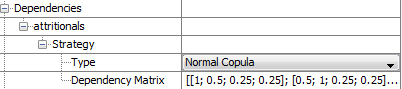
\includegraphics{images/normalCopula1.png}\\[5mm]
		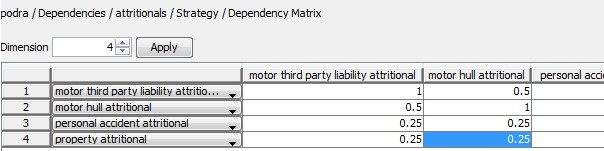
\includegraphics{images/normalCopula2.jpg}
	\caption{4-dimensional normal copula}
	\label{fig:normalCopula}
\end{figure}

It is beyond the scope of this manual to discuss which copula model can be applied in which situation and for what reasons. As demonstrated in Figure~\ref{fig:copulaComparison}, the choice of copula has a major influence on the dependency structure and needs careful consideration.
Figure~\ref{fig:normalCopula} shows a normal copula which correlates four attritional claims generators.

\begin{figure}
		\centering
		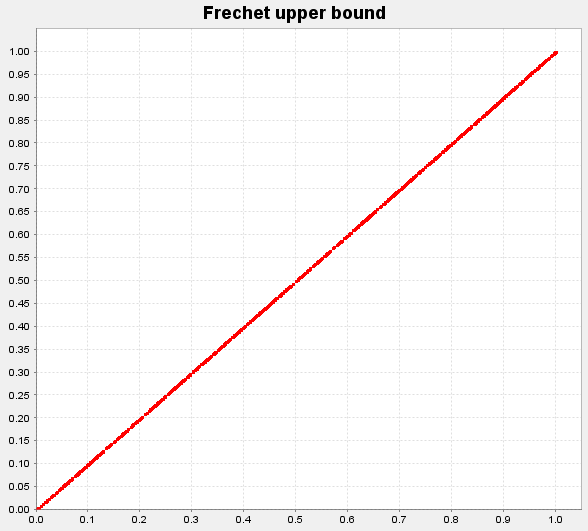
\includegraphics[scale=0.3]{images/FrechetUpperBoundSample.png}		
		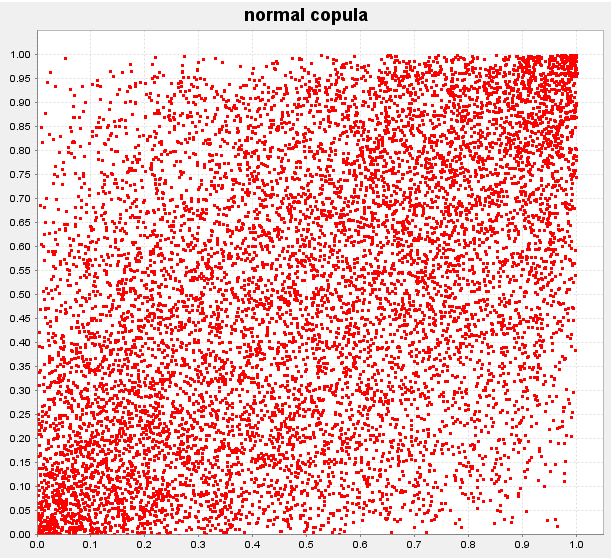
\includegraphics[scale=0.29]{images/normalCopulaSample.png}
		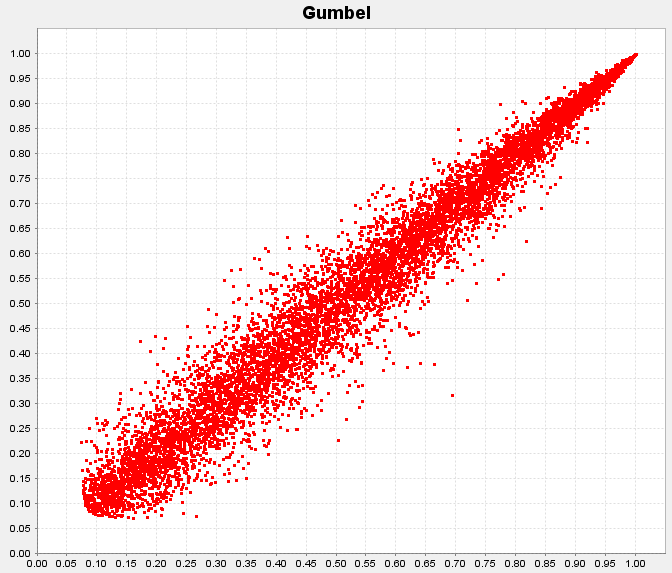
\includegraphics[scale=0.28]{images/GumbelCopulaSample.png}		
	\caption{Comparison of comonotonic, normal and Gumbel copulas}
	\label{fig:copulaComparison}
\end{figure}



\section{Dependency models for single claims}
\label{sec:depSingle}

If we are working with a frequency-severity model to produce single claims, then the most obvious way to correlate these single claims is to postulate a common cause model. In other words, we assume that the claims stem from the same underlying events. This does not imply that the claim sizes must be correlated; but usually this will be the case. Hence, for each iteration we can draw one claims frequency per simulation period for all correlated single claims. And for each of the claim events we can proceed as in the attritional claims case.

It is worthwhile noting that even if some single claims are correlated that does not force us to correlate all single claims. For example, if you work with Poisson distributed claims frequencies, then it is easy to split the frequency into a common event frequency and an idiosyncratic claims frequency. The two average frequencies, the parameters of the Poisson process for the event and the idiosyncratic process, have to add up to the total average frequency. This holds because the sum of two Poisson processes with parameters $\lambda_1$ and $\lambda_2$ is again a Poisson process with parameter $\lambda_1 + \lambda_2$.

\section{A simple dependency example}
\label{sec:depExample}
The following example shows how the above discussed dependency models can be combined in a practical case. It is worthwhile noting that this is a simple example and yet, the resulting correlation structure is already fairly complex. We do not mean to discourage modellers from using such dependency models. But their structure and the calibration of their parameters needs to be carefully reviewed and validated. The limitation of dependency modeling is definitely not a technical one. What can be modelled in RiskAnalytics by far exceeds what most actuaries can soundly explain and validate. Hence, the slogan for dependency modeling should definitely be: Keep it as simple as possible.

Let us assume that we have the two lines of business property and motor hull. For each of these lines of business we model independent large losses using a frequency severity model with Poisson frequency and Pareto severity. The parameters can be seen in the section `Indenpendent LargeLosses' in Figure~\ref{fig:simpleDependencyExample}. 
\begin{figure}
		\centering
		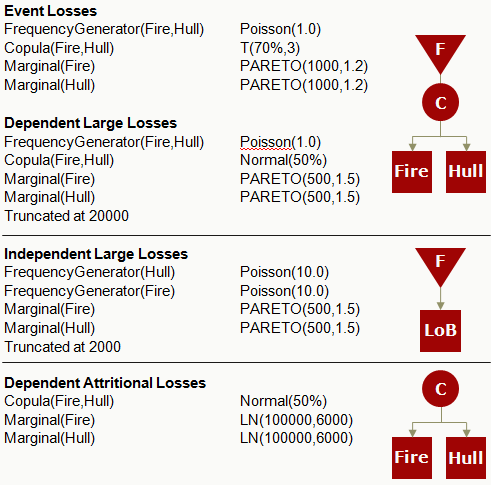
\includegraphics[scale=0.75]{images/twoLoBDependencyExample.png}		
	\caption{Typical dependency structure for two lines of business}
	\label{fig:simpleDependencyExample}
\end{figure}
For the large claims which stem from catastrophic events we assume a common cause model with a Poisson frequency and Pareto severities which are correlated using a student-T copula. Finally, for the attritional claims we use lognormal distributed claims which are correlated using a normal copula. 

This is an absolutely standard dependency structure and the marginal distributions as well as the copulas are not exotic. The resulting aggregate claims have a complex structure as shown in Figure~\ref{fig:simpleDepSample}.  
\begin{figure}
		\centering
		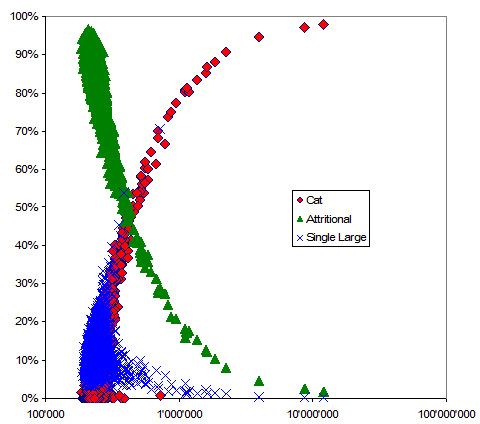
\includegraphics[scale=0.75]{images/simpleDependencySample.png}		
	\caption{Split of the aggregate claims into the three risk types. On the horizontal axis is the claim size in monetary units and the vertical axis is the contribution of each claims type to the aggregate.}
	\label{fig:simpleDepSample}
\end{figure}
For small aggregate claims there are hardly any cat claims involved. With increasing size of the aggregate claims the contribution of the single, non-cat claims and the attritional claims decrease.